% =============================================================================
% Lecture 2: Correlation vs. Causality and Telling Stories with Data
% =============================================================================
\documentclass[9pt,english,aspectratio=169]{beamer}
% =============================================================================
% Pathways: Economics & Finance Workshop — Beamer Preamble
% =============================================================================
% Usage: Each lecture .tex file should start with:
%   \documentclass[10pt,english,aspectratio=169]{beamer}
%   % =============================================================================
% Pathways: Economics & Finance Workshop — Beamer Preamble
% =============================================================================
% Usage: Each lecture .tex file should start with:
%   \documentclass[10pt,english,aspectratio=169]{beamer}
%   % =============================================================================
% Pathways: Economics & Finance Workshop — Beamer Preamble
% =============================================================================
% Usage: Each lecture .tex file should start with:
%   \documentclass[10pt,english,aspectratio=169]{beamer}
%   \input{../../codes/Preambles/header_slides}
% Compile: cd output/Slides && TEXINPUTS=../../codes/Preambles:$TEXINPUTS xelatex file.tex
% =============================================================================

% ---------- Packages ----------
% Fonts
\usepackage{lmodern}
\usepackage[utf8]{inputenc}
\usepackage[normalem]{ulem}

% Math
\usepackage{amsmath,amssymb,amsthm}

% Figures and tables
\usepackage{graphicx}
\usepackage{array,tabularx,booktabs,threeparttable}

% TikZ and pgfplots
\usepackage{pgfplots}
\pgfplotsset{compat=1.18}
\usepackage{tikz}
\usetikzlibrary{positioning,arrows.meta,calc}

% Colored boxes
\usepackage[most]{tcolorbox}

% Miscellaneous
\usepackage{transparent}
\usepackage{setspace}
\usepackage[nodayofweek]{datetime}
\usepackage{hyperref}

% ---------- Theme ----------
\usetheme{CambridgeUS}
\usecolortheme{dolphin}
\usepackage{appendixnumberbeamer}

% ---------- Itemize ----------
\setbeamercovered{invisible}
\setbeamertemplate{itemize items}[default]
\setbeamertemplate{enumerate items}[default]

\setbeamertemplate{itemize item}[triangle]
\setbeamertemplate{itemize subitem}[triangle]
\setbeamertemplate{itemize subsubitem}{-}

% ---------- Headline / Footline ----------
\setbeamertemplate{headline}{}

\setbeamertemplate{footline}{
  \leavevmode
  \hbox{
    \begin{beamercolorbox}[wd=\paperwidth,ht=2.5ex,dp=1.25ex,leftskip=1em,rightskip=1em]{footline}
      \hfill \insertframenumber
    \end{beamercolorbox}
  }
}

\setbeamertemplate{navigation symbols}{}

% ---------- Frame title (centered) ----------
\makeatletter
\setbeamertemplate{frametitle}{
  \nointerlineskip
  \begin{beamercolorbox}[wd=\paperwidth,sep=0.35cm,center]{frametitle}
    {\usebeamerfont{frametitle}\insertframetitle\par}
    \ifx\insertframesubtitle\@empty\else
      \vspace{0.15cm}
      {\usebeamerfont{framesubtitle}\usebeamercolor[fg]{framesubtitle}\insertframesubtitle\par}
    \fi
  \end{beamercolorbox}
}
\makeatother

% ---------- Margins ----------
\setbeamersize{
  text margin left=2em,
  text margin right=2em
}

% ---------- Section outline frames ----------
\AtBeginSection[]{
  \begin{frame}{Outline}
    \tableofcontents[currentsection,
                     currentsubsection,
                     hideothersubsections]
  \end{frame}
}

% =============================================================================
% Colors — Okabe-Ito colorblind-friendly palette
% =============================================================================

\definecolor{black}{HTML}{000000}
\definecolor{orange}{HTML}{E69F00}
\definecolor{skyblue}{HTML}{56B4E9}
\definecolor{green}{HTML}{009E73}
\definecolor{yellow}{HTML}{F0E442}
\definecolor{blue}{HTML}{0072B2}
\definecolor{vermillion}{HTML}{D55E00}
\definecolor{purple}{HTML}{CC79A7}

% Semantic aliases (mapped to Okabe-Ito)
\definecolor{softbg}{HTML}{F5F5F5}
\definecolor{lightgray}{gray}{0.65}

% =============================================================================
% Box Environments
% =============================================================================

% --- Key points (orange background) ---
\newtcolorbox{keybox}{
  colback=orange!12,
  colframe=orange,
  fonttitle=\bfseries,
  boxrule=0.5pt,
  arc=2pt,
  left=6pt,
  right=6pt,
  top=4pt,
  bottom=4pt
}

% --- Highlights (orange left accent) ---
\newtcolorbox{highlightbox}{
  colback=white,
  colframe=orange,
  fonttitle=\bfseries,
  boxrule=0pt,
  leftrule=3pt,
  arc=0pt,
  left=6pt,
  right=6pt,
  top=4pt,
  bottom=4pt
}

% --- Definitions (blue border, titled) ---
\newtcolorbox{definitionbox}[1][]{
  colback=blue!5,
  colframe=blue,
  fonttitle=\bfseries,
  title={#1},
  boxrule=0.5pt,
  arc=2pt,
  left=6pt,
  right=6pt,
  top=4pt,
  bottom=4pt
}

% --- Methods (sky blue background) ---
\newtcolorbox{methodbox}{
  colback=skyblue!8,
  colframe=skyblue!70,
  fonttitle=\bfseries,
  boxrule=0.5pt,
  arc=2pt,
  left=6pt,
  right=6pt,
  top=4pt,
  bottom=4pt
}

% --- Results (green border) ---
\newtcolorbox{resultbox}{
  colback=green!5,
  colframe=green,
  fonttitle=\bfseries,
  boxrule=0.5pt,
  arc=2pt,
  left=6pt,
  right=6pt,
  top=4pt,
  bottom=4pt
}

% --- Quotes (purple left rule) ---
\newtcolorbox{quotebox}{
  colback=softbg,
  colframe=purple,
  fonttitle=\itshape,
  boxrule=0pt,
  leftrule=2pt,
  arc=0pt,
  left=6pt,
  right=6pt,
  top=4pt,
  bottom=4pt
}

% =============================================================================
% Math Commands
% =============================================================================

\newcommand{\E}{\mathrm{E}}
\newcommand{\Var}{\mathrm{Var}}
\newcommand{\Cov}{\mathrm{Cov}}
\newcommand{\R}{\mathbb{R}}
\newcommand{\suminfty}[1]{\sum_{#1=0}^\infty}
\newcommand{\Lcal}{\mathcal{L}}
\newcommand{\prtl}[2]{\frac{\partial #1}{\partial #2}}
\renewcommand{\div}[2]{\frac{d #1}{d #2}}
\newcommand{\suchthat}{\text{ s.t. }}
\newcommand{\wrt}{\text{ w.r.t. }}
\newcommand{\red}[1]{\textcolor{vermillion}{#1}}
\newcommand{\blue}[1]{\textcolor{blue}{#1}}

% =============================================================================
% Economics Shortcuts
% =============================================================================

\newcommand{\OC}{\text{Opportunity Cost}}
\newcommand{\DWL}{\text{DWL}}
\newcommand{\pmark}{\textcolor{resultgreen}{\checkmark}}
\newcommand{\xmark}{\textcolor{darkred}{\texttimes}}

% Compile: cd output/Slides && TEXINPUTS=../../codes/Preambles:$TEXINPUTS xelatex file.tex
% =============================================================================

% ---------- Packages ----------
% Fonts
\usepackage{lmodern}
\usepackage[utf8]{inputenc}
\usepackage[normalem]{ulem}

% Math
\usepackage{amsmath,amssymb,amsthm}

% Figures and tables
\usepackage{graphicx}
\usepackage{array,tabularx,booktabs,threeparttable}

% TikZ and pgfplots
\usepackage{pgfplots}
\pgfplotsset{compat=1.18}
\usepackage{tikz}
\usetikzlibrary{positioning,arrows.meta,calc}

% Colored boxes
\usepackage[most]{tcolorbox}

% Miscellaneous
\usepackage{transparent}
\usepackage{setspace}
\usepackage[nodayofweek]{datetime}
\usepackage{hyperref}

% ---------- Theme ----------
\usetheme{CambridgeUS}
\usecolortheme{dolphin}
\usepackage{appendixnumberbeamer}

% ---------- Itemize ----------
\setbeamercovered{invisible}
\setbeamertemplate{itemize items}[default]
\setbeamertemplate{enumerate items}[default]

\setbeamertemplate{itemize item}[triangle]
\setbeamertemplate{itemize subitem}[triangle]
\setbeamertemplate{itemize subsubitem}{-}

% ---------- Headline / Footline ----------
\setbeamertemplate{headline}{}

\setbeamertemplate{footline}{
  \leavevmode
  \hbox{
    \begin{beamercolorbox}[wd=\paperwidth,ht=2.5ex,dp=1.25ex,leftskip=1em,rightskip=1em]{footline}
      \hfill \insertframenumber
    \end{beamercolorbox}
  }
}

\setbeamertemplate{navigation symbols}{}

% ---------- Frame title (centered) ----------
\makeatletter
\setbeamertemplate{frametitle}{
  \nointerlineskip
  \begin{beamercolorbox}[wd=\paperwidth,sep=0.35cm,center]{frametitle}
    {\usebeamerfont{frametitle}\insertframetitle\par}
    \ifx\insertframesubtitle\@empty\else
      \vspace{0.15cm}
      {\usebeamerfont{framesubtitle}\usebeamercolor[fg]{framesubtitle}\insertframesubtitle\par}
    \fi
  \end{beamercolorbox}
}
\makeatother

% ---------- Margins ----------
\setbeamersize{
  text margin left=2em,
  text margin right=2em
}

% ---------- Section outline frames ----------
\AtBeginSection[]{
  \begin{frame}{Outline}
    \tableofcontents[currentsection,
                     currentsubsection,
                     hideothersubsections]
  \end{frame}
}

% =============================================================================
% Colors — Okabe-Ito colorblind-friendly palette
% =============================================================================

\definecolor{black}{HTML}{000000}
\definecolor{orange}{HTML}{E69F00}
\definecolor{skyblue}{HTML}{56B4E9}
\definecolor{green}{HTML}{009E73}
\definecolor{yellow}{HTML}{F0E442}
\definecolor{blue}{HTML}{0072B2}
\definecolor{vermillion}{HTML}{D55E00}
\definecolor{purple}{HTML}{CC79A7}

% Semantic aliases (mapped to Okabe-Ito)
\definecolor{softbg}{HTML}{F5F5F5}
\definecolor{lightgray}{gray}{0.65}

% =============================================================================
% Box Environments
% =============================================================================

% --- Key points (orange background) ---
\newtcolorbox{keybox}{
  colback=orange!12,
  colframe=orange,
  fonttitle=\bfseries,
  boxrule=0.5pt,
  arc=2pt,
  left=6pt,
  right=6pt,
  top=4pt,
  bottom=4pt
}

% --- Highlights (orange left accent) ---
\newtcolorbox{highlightbox}{
  colback=white,
  colframe=orange,
  fonttitle=\bfseries,
  boxrule=0pt,
  leftrule=3pt,
  arc=0pt,
  left=6pt,
  right=6pt,
  top=4pt,
  bottom=4pt
}

% --- Definitions (blue border, titled) ---
\newtcolorbox{definitionbox}[1][]{
  colback=blue!5,
  colframe=blue,
  fonttitle=\bfseries,
  title={#1},
  boxrule=0.5pt,
  arc=2pt,
  left=6pt,
  right=6pt,
  top=4pt,
  bottom=4pt
}

% --- Methods (sky blue background) ---
\newtcolorbox{methodbox}{
  colback=skyblue!8,
  colframe=skyblue!70,
  fonttitle=\bfseries,
  boxrule=0.5pt,
  arc=2pt,
  left=6pt,
  right=6pt,
  top=4pt,
  bottom=4pt
}

% --- Results (green border) ---
\newtcolorbox{resultbox}{
  colback=green!5,
  colframe=green,
  fonttitle=\bfseries,
  boxrule=0.5pt,
  arc=2pt,
  left=6pt,
  right=6pt,
  top=4pt,
  bottom=4pt
}

% --- Quotes (purple left rule) ---
\newtcolorbox{quotebox}{
  colback=softbg,
  colframe=purple,
  fonttitle=\itshape,
  boxrule=0pt,
  leftrule=2pt,
  arc=0pt,
  left=6pt,
  right=6pt,
  top=4pt,
  bottom=4pt
}

% =============================================================================
% Math Commands
% =============================================================================

\newcommand{\E}{\mathrm{E}}
\newcommand{\Var}{\mathrm{Var}}
\newcommand{\Cov}{\mathrm{Cov}}
\newcommand{\R}{\mathbb{R}}
\newcommand{\suminfty}[1]{\sum_{#1=0}^\infty}
\newcommand{\Lcal}{\mathcal{L}}
\newcommand{\prtl}[2]{\frac{\partial #1}{\partial #2}}
\renewcommand{\div}[2]{\frac{d #1}{d #2}}
\newcommand{\suchthat}{\text{ s.t. }}
\newcommand{\wrt}{\text{ w.r.t. }}
\newcommand{\red}[1]{\textcolor{vermillion}{#1}}
\newcommand{\blue}[1]{\textcolor{blue}{#1}}

% =============================================================================
% Economics Shortcuts
% =============================================================================

\newcommand{\OC}{\text{Opportunity Cost}}
\newcommand{\DWL}{\text{DWL}}
\newcommand{\pmark}{\textcolor{resultgreen}{\checkmark}}
\newcommand{\xmark}{\textcolor{darkred}{\texttimes}}

% Compile: cd output/Slides && TEXINPUTS=../../codes/Preambles:$TEXINPUTS xelatex file.tex
% =============================================================================

% ---------- Packages ----------
% Fonts
\usepackage{lmodern}
\usepackage[utf8]{inputenc}
\usepackage[normalem]{ulem}

% Math
\usepackage{amsmath,amssymb,amsthm}

% Figures and tables
\usepackage{graphicx}
\usepackage{array,tabularx,booktabs,threeparttable}

% TikZ and pgfplots
\usepackage{pgfplots}
\pgfplotsset{compat=1.18}
\usepackage{tikz}
\usetikzlibrary{positioning,arrows.meta,calc}

% Colored boxes
\usepackage[most]{tcolorbox}

% Miscellaneous
\usepackage{transparent}
\usepackage{setspace}
\usepackage[nodayofweek]{datetime}
\usepackage{hyperref}

% ---------- Theme ----------
\usetheme{CambridgeUS}
\usecolortheme{dolphin}
\usepackage{appendixnumberbeamer}

% ---------- Itemize ----------
\setbeamercovered{invisible}
\setbeamertemplate{itemize items}[default]
\setbeamertemplate{enumerate items}[default]

\setbeamertemplate{itemize item}[triangle]
\setbeamertemplate{itemize subitem}[triangle]
\setbeamertemplate{itemize subsubitem}{-}

% ---------- Headline / Footline ----------
\setbeamertemplate{headline}{}

\setbeamertemplate{footline}{
  \leavevmode
  \hbox{
    \begin{beamercolorbox}[wd=\paperwidth,ht=2.5ex,dp=1.25ex,leftskip=1em,rightskip=1em]{footline}
      \hfill \insertframenumber
    \end{beamercolorbox}
  }
}

\setbeamertemplate{navigation symbols}{}

% ---------- Frame title (centered) ----------
\makeatletter
\setbeamertemplate{frametitle}{
  \nointerlineskip
  \begin{beamercolorbox}[wd=\paperwidth,sep=0.35cm,center]{frametitle}
    {\usebeamerfont{frametitle}\insertframetitle\par}
    \ifx\insertframesubtitle\@empty\else
      \vspace{0.15cm}
      {\usebeamerfont{framesubtitle}\usebeamercolor[fg]{framesubtitle}\insertframesubtitle\par}
    \fi
  \end{beamercolorbox}
}
\makeatother

% ---------- Margins ----------
\setbeamersize{
  text margin left=2em,
  text margin right=2em
}

% ---------- Section outline frames ----------
\AtBeginSection[]{
  \begin{frame}{Outline}
    \tableofcontents[currentsection,
                     currentsubsection,
                     hideothersubsections]
  \end{frame}
}

% =============================================================================
% Colors — Okabe-Ito colorblind-friendly palette
% =============================================================================

\definecolor{black}{HTML}{000000}
\definecolor{orange}{HTML}{E69F00}
\definecolor{skyblue}{HTML}{56B4E9}
\definecolor{green}{HTML}{009E73}
\definecolor{yellow}{HTML}{F0E442}
\definecolor{blue}{HTML}{0072B2}
\definecolor{vermillion}{HTML}{D55E00}
\definecolor{purple}{HTML}{CC79A7}

% Semantic aliases (mapped to Okabe-Ito)
\definecolor{softbg}{HTML}{F5F5F5}
\definecolor{lightgray}{gray}{0.65}

% =============================================================================
% Box Environments
% =============================================================================

% --- Key points (orange background) ---
\newtcolorbox{keybox}{
  colback=orange!12,
  colframe=orange,
  fonttitle=\bfseries,
  boxrule=0.5pt,
  arc=2pt,
  left=6pt,
  right=6pt,
  top=4pt,
  bottom=4pt
}

% --- Highlights (orange left accent) ---
\newtcolorbox{highlightbox}{
  colback=white,
  colframe=orange,
  fonttitle=\bfseries,
  boxrule=0pt,
  leftrule=3pt,
  arc=0pt,
  left=6pt,
  right=6pt,
  top=4pt,
  bottom=4pt
}

% --- Definitions (blue border, titled) ---
\newtcolorbox{definitionbox}[1][]{
  colback=blue!5,
  colframe=blue,
  fonttitle=\bfseries,
  title={#1},
  boxrule=0.5pt,
  arc=2pt,
  left=6pt,
  right=6pt,
  top=4pt,
  bottom=4pt
}

% --- Methods (sky blue background) ---
\newtcolorbox{methodbox}{
  colback=skyblue!8,
  colframe=skyblue!70,
  fonttitle=\bfseries,
  boxrule=0.5pt,
  arc=2pt,
  left=6pt,
  right=6pt,
  top=4pt,
  bottom=4pt
}

% --- Results (green border) ---
\newtcolorbox{resultbox}{
  colback=green!5,
  colframe=green,
  fonttitle=\bfseries,
  boxrule=0.5pt,
  arc=2pt,
  left=6pt,
  right=6pt,
  top=4pt,
  bottom=4pt
}

% --- Quotes (purple left rule) ---
\newtcolorbox{quotebox}{
  colback=softbg,
  colframe=purple,
  fonttitle=\itshape,
  boxrule=0pt,
  leftrule=2pt,
  arc=0pt,
  left=6pt,
  right=6pt,
  top=4pt,
  bottom=4pt
}

% =============================================================================
% Math Commands
% =============================================================================

\newcommand{\E}{\mathrm{E}}
\newcommand{\Var}{\mathrm{Var}}
\newcommand{\Cov}{\mathrm{Cov}}
\newcommand{\R}{\mathbb{R}}
\newcommand{\suminfty}[1]{\sum_{#1=0}^\infty}
\newcommand{\Lcal}{\mathcal{L}}
\newcommand{\prtl}[2]{\frac{\partial #1}{\partial #2}}
\renewcommand{\div}[2]{\frac{d #1}{d #2}}
\newcommand{\suchthat}{\text{ s.t. }}
\newcommand{\wrt}{\text{ w.r.t. }}
\newcommand{\red}[1]{\textcolor{vermillion}{#1}}
\newcommand{\blue}[1]{\textcolor{blue}{#1}}

% =============================================================================
% Economics Shortcuts
% =============================================================================

\newcommand{\OC}{\text{Opportunity Cost}}
\newcommand{\DWL}{\text{DWL}}
\newcommand{\pmark}{\textcolor{resultgreen}{\checkmark}}
\newcommand{\xmark}{\textcolor{darkred}{\texttimes}}


% ---------- Placeholder for missing images ----------
\newcommand{\placeholderimg}[2][width=\textwidth]{%
  \IfFileExists{#2}{%
    \includegraphics[#1]{#2}%
  }{%
    \fcolorbox{gray!30}{gray!10}{\parbox{3.8cm}{\centering\vspace{0.8cm}{\tiny\itshape\textcolor{gray}{placeholder}}\vspace{0.8cm}}}%
  }%
}

% ---------- Title ----------
\title{\textbf{Correlation vs.\ Causality}}
\subtitle{Pathways to Arts \& Humanities Summer Scholars Program}
\author{Instructor: Tudor Schlanger}
\date{Summer 2026}

\begin{document}

% =============================================================================
% Title
% =============================================================================
\begin{frame}
  \titlepage
\end{frame}

\begin{frame}{Review: Opportunity Cost}

  \begin{questionbox}
    You won a \textbf{free ticket} to see an Eric Clapton concert (which has no
    resale value). Bob Dylan is performing on the same night and is your
    next-best alternative activity. Tickets to see Dylan cost \textbf{\$40}. On
    any given day, you would be willing to pay up to \textbf{\$50} to see Dylan.
    Assume there are no other costs of seeing either performer.

    \vspace{0.5em}
    Based on this information, what is the \textbf{opportunity cost} of seeing
    Eric Clapton?
  \end{questionbox}

  \vspace{0.6em}
  \begin{enumerate}[A.]
    \item \$0
    \item \$10
    \item \$40
    \item \$50
  \end{enumerate}

\end{frame}

\begin{frame}{Review: Opportunity Cost --- Answer}

  \begin{answerbox}
    The correct answer is \textbf{B. \$10}.\\[0.5em]
    The opportunity cost of seeing Clapton is what you \textbf{give up}: the net benefit of seeing Dylan.\\[0.3em]
    You value Dylan at \$50 and the ticket costs \$40, so the opportunity cost is \$50 $-$ \$40 $=$ \textbf{\$10}.
  \end{answerbox}

\end{frame}

% =============================================================================
\section{Can You Trust What You See?}
% =============================================================================

\begin{frame}{The Cat Question}

  \begin{columns}[T]
    \begin{column}{0.58\textwidth}
      \vspace{1em}
      \begin{questionbox}
        Did the cat leave a dent?
      \end{questionbox}
    \end{column}
    \begin{column}{0.38\textwidth}
      \vspace{1em}
      \placeholderimg{fig/cat_roof.jpg}

      \vspace{0.3em}
      {\tiny\textcolor{lightgray}{Photo: Internet (fair use, educational)}}
    \end{column}
  \end{columns}

\end{frame}

\begin{frame}{Catchy Headlines}

  \begin{columns}[T]
    \begin{column}{0.58\textwidth}
      \begin{questionbox}
        A 2012 TIME Magazine headline reads:\\[0.3em]
        {\large \textbf{\href{https://healthland.time.com/2012/07/11/alcohol-does-a-body-good-study-finds-it-boosts-bone-health/}{``Alcohol Does a Body Good? Study Finds It Boosts Bone Health''}}}\\[0.3em]
        Does this mean drinking alcohol strengthens your bones?
      \end{questionbox}
    \end{column}
    \begin{column}{0.38\textwidth}
      \vspace{1em}
      \placeholderimg{fig/wine_glass.jpg}

      \vspace{0.3em}
      {\tiny\textcolor{lightgray}{Photo: Pexels (free license)}}
    \end{column}
  \end{columns}

\end{frame}

\begin{frame}{Today's Agenda}

  \vspace{1em}
  By the end of this class, you will be \textbf{harder to fool}!

  \vspace{1em}
  {Three things we will practice:}

  \vspace{0.5em}
  \begin{enumerate}
    \item \textbf{Correlation vs.\ causality}: how to tell the difference
    \item \textbf{Misleading graphs}: how data can make you think it's causality!
    \item \textbf{Chart detective}: how to protect yourself in the future
  \end{enumerate}

\end{frame}

% =============================================================================
\section{Correlation vs.\ Causality}
% =============================================================================

\begin{frame}{A Suspicious Pattern}

  \centering
  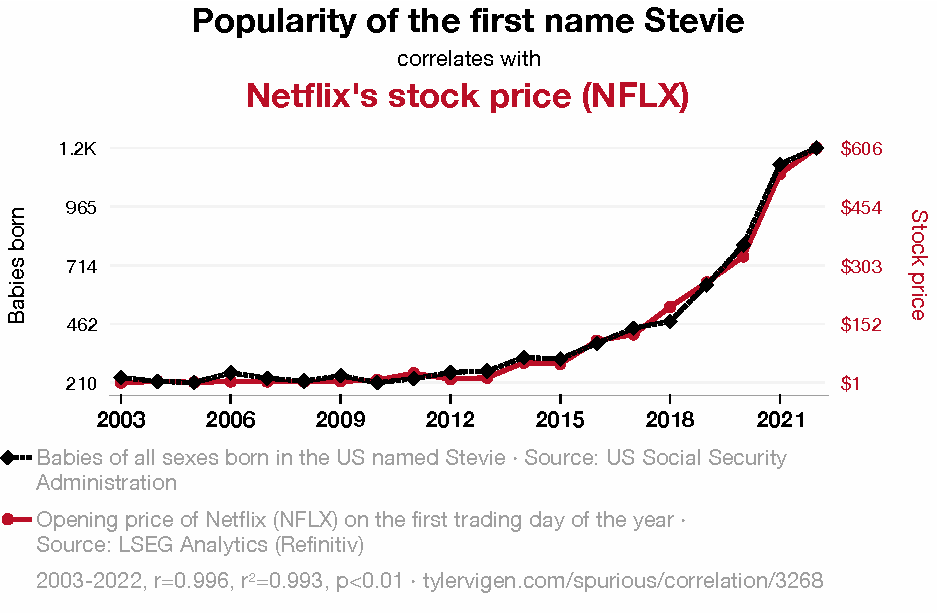
\includegraphics[width=0.85\textwidth, height=6.5cm, keepaspectratio]{fig/stevie_netflix.pdf}

  \vspace{0.3em}
  {\tiny\textcolor{lightgray}{Source: tylervigen.com --- Spurious Correlations.}}

\end{frame}

\begin{frame}{What's Going On?}

  \begin{questionbox}
    Does the popularity of the name ``Stevie'' \textbf{cause} Netflix's stock price to rise?\\[0.3em]
    In your group, come up with:
    \begin{enumerate}
      \item One \textbf{funny} explanation (technically possible but absurd)
      \item One sentence explaining why the chart \textbf{does not prove} causality
    \end{enumerate}
  \end{questionbox}

  \vspace{0.8em}
  \Large\textcolor{blue}{Discuss with your group for 1 minute \ldots}

\end{frame}

\begin{frame}{What's Going On?}

  \begin{answerbox}
    The chart shows a \textbf{pattern}, not a cause.\\[0.3em]
    Both the name ``Stevie'' and Netflix's stock price were rising over the same period---likely for completely unrelated reasons.
  \end{answerbox}

  \vspace{0.5em}
  \textbf{\emph{Two things trending together does not mean one caused the other.}} Time itself can create fake-looking relationships.

\end{frame}

\begin{frame}{Correlation}

  \begin{columns}[T]
    \begin{column}{0.48\textwidth}
      \begin{definitionbox}[Correlation]
        Two things \textbf{move together}---when one goes up, the other tends to go up (or down).\\[0.3em]
        It tells us there is a \textbf{pattern}, but \textbf{not why} the pattern exists.
      \end{definitionbox}

      \vspace{0.5em}
      % {\small \textbf{Example:} Ice cream sales and heatstroke cases both rise in summer.}
    \end{column}
    \begin{column}{0.48\textwidth}
      \pause
      \vspace{1em}
      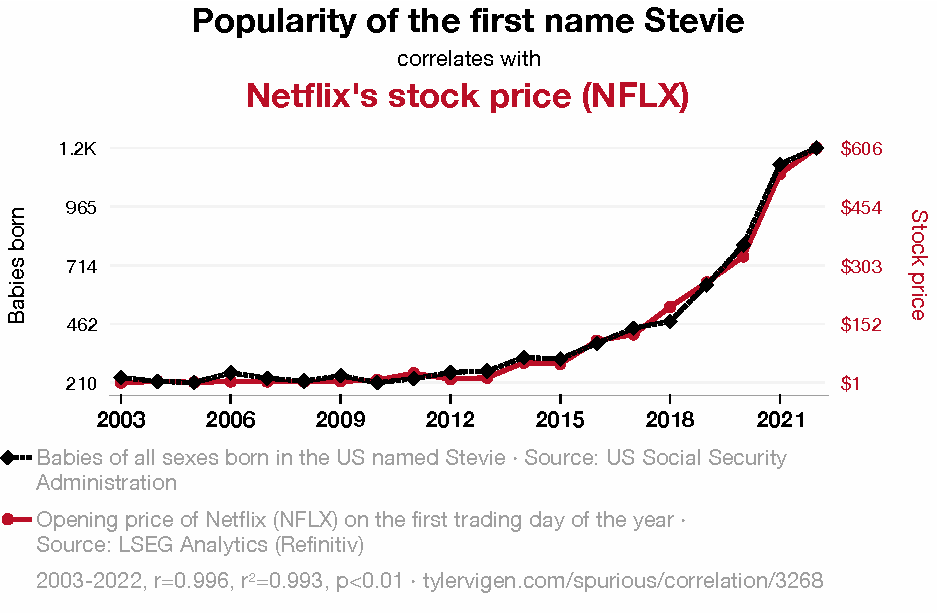
\includegraphics[width=\textwidth]{fig/stevie_netflix.pdf}

      \vspace{0.3em}
      {\tiny\textcolor{lightgray}{Source: tylervigen.com}}
    \end{column}
  \end{columns}

\end{frame}

\begin{frame}{Correlation: Scatter Plot}

  \begin{columns}[T]
    \begin{column}{0.48\textwidth}
      \begin{definitionbox}[Correlation]
        Two things \textbf{move together}---when one goes up, the other tends to go up (or down).\\[0.3em]
        It tells us there is a \textbf{pattern}, but \textbf{not why} the pattern exists.
      \end{definitionbox}

      \vspace{0.5em}
      {\small Does Netflix \textbf{cause} babies to be named Stevie?}
    \end{column}
    \begin{column}{0.48\textwidth}
      \centering
      \begin{tikzpicture}
        \begin{axis}[
          width=\textwidth,
          height=6.5cm,
          xlabel={\small Netflix stock price (\$)},
          ylabel={\small Babies named ``Stevie''},
          xmin=-20, xmax=680,
          ymin=150, ymax=1350,
          grid=major,
          grid style={gray!20},
          xticklabel style={font=\tiny},
          yticklabel style={font=\tiny},
          xlabel style={font=\small},
          ylabel style={font=\small},
        ]
        \addplot[only marks, mark=*, mark size=2pt, blue!70!black] coordinates {
          (1,232) (4,215) (2,211) (4,251) (4,229)
          (4,217) (4,239) (8,210) (25,227) (10,253)
          (14,259) (52,316) (49,310) (109,376) (125,440)
          (196,469) (259,622) (326,791) (539,1131) (606,1200)
        };
        % Line of best fit (r = 0.996)
        \addplot[domain=0:650, thick, vermillion, dashed, samples=2] {232 + 1.6*x};
        % Year annotations
        \node[font=\tiny, anchor=south] at (1,240) {03};
        \node[font=\tiny, anchor=west] at (6,215) {04};
        \node[font=\tiny, anchor=north] at (2,203) {05};
        \node[font=\tiny, anchor=west] at (6,251) {06};
        \node[font=\tiny, anchor=south west] at (6,229) {07};
        \node[font=\tiny, anchor=north] at (4,209) {08};
        \node[font=\tiny, anchor=south] at (4,247) {09};
        \node[font=\tiny, anchor=north west] at (10,205) {10};
        \node[font=\tiny, anchor=south west] at (27,227) {11};
        \node[font=\tiny, anchor=west] at (12,253) {12};
        \node[font=\tiny, anchor=south west] at (16,259) {13};
        \node[font=\tiny, anchor=south] at (52,324) {14};
        \node[font=\tiny, anchor=north] at (49,302) {15};
        \node[font=\tiny, anchor=south] at (109,384) {16};
        \node[font=\tiny, anchor=south] at (125,448) {17};
        \node[font=\tiny, anchor=south] at (196,477) {18};
        \node[font=\tiny, anchor=south] at (259,630) {19};
        \node[font=\tiny, anchor=south] at (326,799) {20};
        \node[font=\tiny, anchor=south] at (539,1139) {21};
        \node[font=\tiny, anchor=south] at (606,1208) {22};
        \end{axis}
      \end{tikzpicture}
    \end{column}
  \end{columns}

\end{frame}

\begin{frame}{Why Do Correlations Happen?}

  \begin{columns}[T]
    \begin{column}{0.48\textwidth}
      There are \textbf{four} possible explanations when you see two things moving together:

      \vspace{0.8em}
      \begin{enumerate}
        \item \textcolor{vermillion}{\textbf{Coincidence}}
        \item \textcolor{green}{\textbf{Causality}}
        \item \textcolor{blue}{\textbf{Reverse causality}}
        \item \textcolor{orange}{\textbf{Hidden third factor (confounder)}}
      \end{enumerate}
    \end{column}
    \begin{column}{0.48\textwidth}
      \centering
      \begin{tikzpicture}
        \begin{axis}[
          width=\textwidth,
          height=6.5cm,
          xlabel={\small Netflix stock price (\$)},
          ylabel={\small Babies named ``Stevie''},
          xmin=-20, xmax=680,
          ymin=150, ymax=1350,
          grid=major,
          grid style={gray!20},
          xticklabel style={font=\tiny},
          yticklabel style={font=\tiny},
          xlabel style={font=\small},
          ylabel style={font=\small},
        ]
        \addplot[only marks, mark=*, mark size=2pt, blue!70!black] coordinates {
          (1,232) (4,215) (2,211) (4,251) (4,229)
          (4,217) (4,239) (8,210) (25,227) (10,253)
          (14,259) (52,316) (49,310) (109,376) (125,440)
          (196,469) (259,622) (326,791) (539,1131) (606,1200)
        };
        % Line of best fit (r = 0.996)
        \addplot[domain=0:650, thick, vermillion, dashed, samples=2] {232 + 1.6*x};
        % Year annotations
        \node[font=\tiny, anchor=south] at (1,240) {03};
        \node[font=\tiny, anchor=west] at (6,215) {04};
        \node[font=\tiny, anchor=north] at (2,203) {05};
        \node[font=\tiny, anchor=west] at (6,251) {06};
        \node[font=\tiny, anchor=south west] at (6,229) {07};
        \node[font=\tiny, anchor=north] at (4,209) {08};
        \node[font=\tiny, anchor=south] at (4,247) {09};
        \node[font=\tiny, anchor=north west] at (10,205) {10};
        \node[font=\tiny, anchor=south west] at (27,227) {11};
        \node[font=\tiny, anchor=west] at (12,253) {12};
        \node[font=\tiny, anchor=south west] at (16,259) {13};
        \node[font=\tiny, anchor=south] at (52,324) {14};
        \node[font=\tiny, anchor=north] at (49,302) {15};
        \node[font=\tiny, anchor=south] at (109,384) {16};
        \node[font=\tiny, anchor=south] at (125,448) {17};
        \node[font=\tiny, anchor=south] at (196,477) {18};
        \node[font=\tiny, anchor=south] at (259,630) {19};
        \node[font=\tiny, anchor=south] at (326,799) {20};
        \node[font=\tiny, anchor=south] at (539,1139) {21};
        \node[font=\tiny, anchor=south] at (606,1208) {22};
        \end{axis}
      \end{tikzpicture}
    \end{column}
  \end{columns}

\end{frame}

\begin{frame}{Causality}

  \begin{columns}[T]
    \begin{column}{0.48\textwidth}
      \begin{definitionbox}[Causality]
        One thing actually \textbf{changes} another.\\[0.3em]
        If you change A, it \textbf{affects} B.
      \end{definitionbox}

      \vspace{0.5em}
      % {\small \textbf{Example:} Hot weather causes heatstroke. (Not the reverse.)}
    \end{column}
    \begin{column}{0.48\textwidth}
      \vspace{0.5em} \pause 
      {\small\textbf{Everyday examples:}}

      \vspace{0.5em}
      \begin{itemize}
        \item Flipping a light switch $\rightarrow$ light turns on
        \item Studying more $\rightarrow$ higher test scores
        \item Drinking coffee $\rightarrow$ feeling more alert

      \end{itemize}

      \vspace{0.5em}
      {\small In each case, changing one thing \textbf{directly affects} the other.}
    \end{column}
      % --- Heatwave figure (commented out) ---
      % \centering
      % {\scriptsize\textbf{France, August 2003 Heatwave}}
      % \begin{tikzpicture} ... \end{tikzpicture}
      % {\tiny\textcolor{lightgray}{Data: Fouillet et al.\ (2006)}}
  \end{columns}

\end{frame}

\begin{frame}{DAGs: A Thinking Tool}

  \begin{columns}[T]
    \begin{column}{0.58\textwidth}
      A \textbf{DAG} (\textbf{D}irected \textbf{A}cyclic \textbf{G}raph) is a map of what causes what.

      \vspace{0.5em}
      Drawing the arrows forces you to think about:
      \begin{itemize}
        \item \textbf{Direction}---which way does causality flow?
        % \item \textbf{Hidden factors}---is there a confounder I'm missing?
        \item \textbf{What's real}---which connections are causal vs.\ just correlated?
      \end{itemize}

      \vspace{0.5em}
      Economists and scientists use DAGs to reason carefully about cause and effect.
    \end{column}
    \begin{column}{0.38\textwidth}
      \vspace{1em}
      \centering
      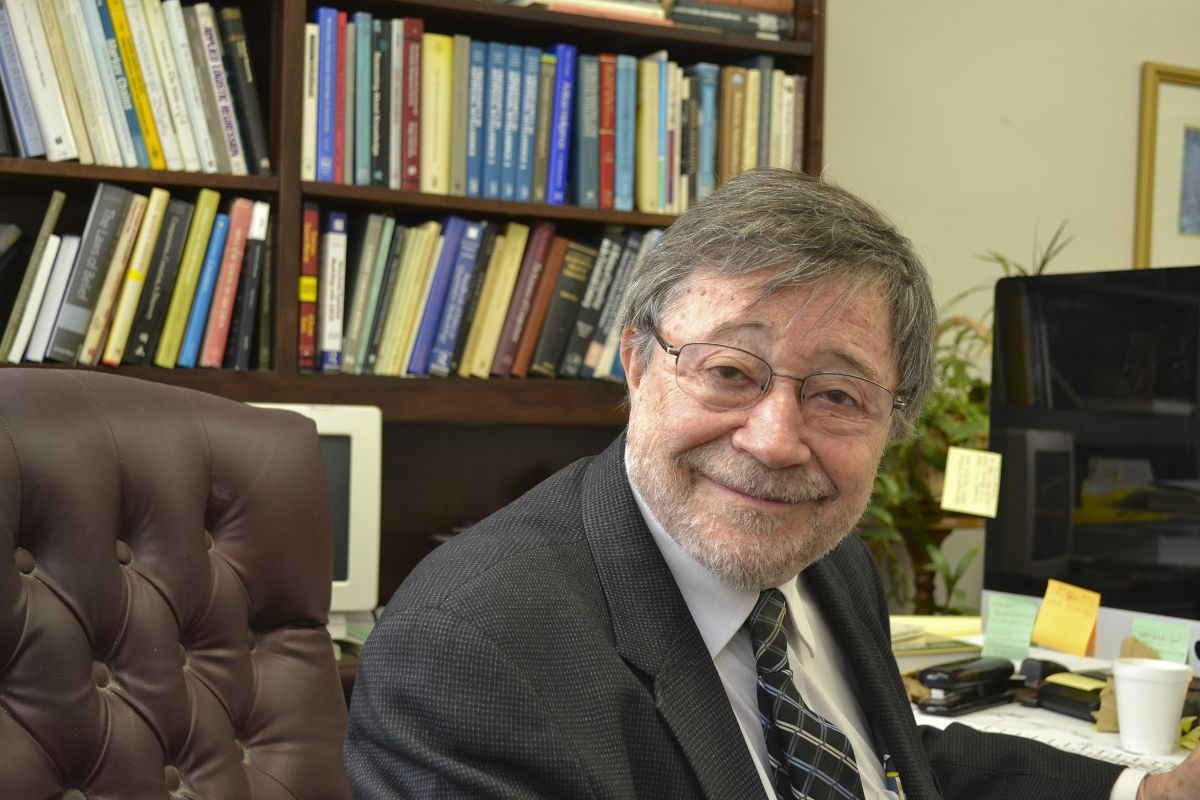
\includegraphics[width=\textwidth, height=5cm, keepaspectratio]{fig/judea_pearl.jpg}

      \vspace{0.3em}
      {\small\textbf{Judea Pearl}}\\
      {\tiny Turing Award winner (2011)\\Pioneered causal DAGs}

      \vspace{0.2em}
      {\tiny\textcolor{lightgray}{Photo: UCLA Newsroom}}
    \end{column}
  \end{columns}

\end{frame}

\begin{frame}{DAGs: The Simplest Case}

  \centering
  \vspace{2em}
  \begin{tikzpicture}[
    node distance=2cm and 4cm,
    box/.style={draw, rounded corners=4pt, fill=blue!8, minimum width=2.5cm, minimum height=1cm, align=center, font=\normalsize},
    arr/.style={-{Stealth[length=7pt]}, thick, blue!70}
  ]
    \node[box] (a) {\textbf{Event A}};
    \node[box, right=4cm of a] (b) {\textbf{Event B}};

    \draw[arr] (a) -- node[above, font=\small] {causes} (b);
  \end{tikzpicture}

  \vspace{1.5em}
  \begin{insightbox}
    The arrow means: if you \textbf{change} A, B changes too. \\ The direction matters: A $\rightarrow$ B is not the same as B $\rightarrow$ A.
  \end{insightbox}

\end{frame}

\begin{frame}{Why Do Correlations Happen?}

  \begin{columns}[T]
    \begin{column}{0.48\textwidth}
      There are \textbf{four} possible explanations when you see two things moving together:

      \vspace{0.8em}
      \begin{enumerate}
        \item \textcolor{vermillion}{\textbf{Coincidence}}
        \item \textcolor{green}{\textbf{Causality}}
        \item \textcolor{blue}{\textbf{Reverse causality}}
        \item \textcolor{orange}{\textbf{Hidden third factor (confounder)}}
      \end{enumerate}
    \end{column}
    \begin{column}{0.48\textwidth}
      \centering
      \begin{tikzpicture}
        \begin{axis}[
          width=\textwidth,
          height=6.5cm,
          xlabel={\small Netflix stock price (\$)},
          ylabel={\small Babies named ``Stevie''},
          xmin=-20, xmax=680,
          ymin=150, ymax=1350,
          grid=major,
          grid style={gray!20},
          xticklabel style={font=\tiny},
          yticklabel style={font=\tiny},
          xlabel style={font=\small},
          ylabel style={font=\small},
        ]
        \addplot[only marks, mark=*, mark size=2pt, blue!70!black] coordinates {
          (1,232) (4,215) (2,211) (4,251) (4,229)
          (4,217) (4,239) (8,210) (25,227) (10,253)
          (14,259) (52,316) (49,310) (109,376) (125,440)
          (196,469) (259,622) (326,791) (539,1131) (606,1200)
        };
        % Line of best fit (r = 0.996)
        \addplot[domain=0:650, thick, vermillion, dashed, samples=2] {232 + 1.6*x};
        % Year annotations
        \node[font=\tiny, anchor=south] at (1,240) {03};
        \node[font=\tiny, anchor=west] at (6,215) {04};
        \node[font=\tiny, anchor=north] at (2,203) {05};
        \node[font=\tiny, anchor=west] at (6,251) {06};
        \node[font=\tiny, anchor=south west] at (6,229) {07};
        \node[font=\tiny, anchor=north] at (4,209) {08};
        \node[font=\tiny, anchor=south] at (4,247) {09};
        \node[font=\tiny, anchor=north west] at (10,205) {10};
        \node[font=\tiny, anchor=south west] at (27,227) {11};
        \node[font=\tiny, anchor=west] at (12,253) {12};
        \node[font=\tiny, anchor=south west] at (16,259) {13};
        \node[font=\tiny, anchor=south] at (52,324) {14};
        \node[font=\tiny, anchor=north] at (49,302) {15};
        \node[font=\tiny, anchor=south] at (109,384) {16};
        \node[font=\tiny, anchor=south] at (125,448) {17};
        \node[font=\tiny, anchor=south] at (196,477) {18};
        \node[font=\tiny, anchor=south] at (259,630) {19};
        \node[font=\tiny, anchor=south] at (326,799) {20};
        \node[font=\tiny, anchor=south] at (539,1139) {21};
        \node[font=\tiny, anchor=south] at (606,1208) {22};
        \end{axis}
      \end{tikzpicture}
    \end{column}
  \end{columns}

\end{frame}

\begin{frame}{DAGs: Reverse Causality}

  \centering
  \vspace{2em}
  \begin{tikzpicture}[
    node distance=2cm and 4cm,
    box/.style={draw, rounded corners=4pt, fill=blue!8, minimum width=2.5cm, minimum height=1cm, align=center, font=\normalsize},
    arr/.style={-{Stealth[length=7pt]}, thick, blue!70}
  ]
    \node[box] (a) {\textbf{Event A}};
    \node[box, right=4cm of a] (b) {\textbf{Event B}};

    \draw[arr] (b) -- node[above, font=\small] {causes} (a);
  \end{tikzpicture}

  \vspace{1.5em}
  \begin{insightbox}
    You \emph{think} A causes B, but the arrow actually runs the other way: \textbf{B causes A}. Getting the direction wrong leads to the wrong conclusion.
  \end{insightbox}

\end{frame}

\begin{frame}{DAGs: Reverse Causality --- Example}

  \centering
  \vspace{2em}
  \begin{tikzpicture}[
    node distance=2cm and 4cm,
    box/.style={draw, rounded corners=4pt, fill=blue!8, minimum width=3.5cm, minimum height=1cm, align=center, font=\normalsize},
  ]
    \node[box] (a) {\textbf{Student gets}\\[0.2em]\textbf{tutoring}};
    \node[box, right=4cm of a] (b) {\textbf{Student gets}\\[0.2em]\textbf{low grades}};
  \end{tikzpicture}

\end{frame}

\begin{frame}{DAGs: Reverse Causality --- Example}

  \centering
  \vspace{2em}
  \begin{tikzpicture}[
    node distance=2cm and 4cm,
    box/.style={draw, rounded corners=4pt, fill=blue!8, minimum width=3.5cm, minimum height=1cm, align=center, font=\normalsize},
    arr/.style={-{Stealth[length=7pt]}, thick, blue!70}
  ]
    \node[box] (a) {\textbf{Student gets}\\[0.2em]\textbf{tutoring}};
    \node[box, right=4cm of a] (b) {\textbf{Student gets}\\[0.2em]\textbf{low grades}};

    \draw[arr] (b) -- node[above, font=\small] {causes} (a);
  \end{tikzpicture}

  \vspace{1.5em}
  \begin{insightbox}
    Students who get tutoring have lower grades. Does tutoring \textbf{cause} bad grades? No---students who are \textbf{already struggling} are the ones who seek tutoring.
  \end{insightbox}

\end{frame}

\begin{frame}{Why Do Correlations Happen?}

  \begin{columns}[T]
    \begin{column}{0.48\textwidth}
      There are \textbf{four} possible explanations when you see two things moving together:

      \vspace{0.8em}
      \begin{enumerate}
        \item \textcolor{vermillion}{\textbf{Coincidence}}
        \item \textcolor{green}{\textbf{Causality}}
        \item \textcolor{blue}{\textbf{Reverse causality}}
        \item \textcolor{orange}{\textbf{Hidden third factor (confounder)}}
      \end{enumerate}
    \end{column}
    \begin{column}{0.48\textwidth}
      \centering
      \begin{tikzpicture}
        \begin{axis}[
          width=\textwidth,
          height=6.5cm,
          xlabel={\small Netflix stock price (\$)},
          ylabel={\small Babies named ``Stevie''},
          xmin=-20, xmax=680,
          ymin=150, ymax=1350,
          grid=major,
          grid style={gray!20},
          xticklabel style={font=\tiny},
          yticklabel style={font=\tiny},
          xlabel style={font=\small},
          ylabel style={font=\small},
        ]
        \addplot[only marks, mark=*, mark size=2pt, blue!70!black] coordinates {
          (1,232) (4,215) (2,211) (4,251) (4,229)
          (4,217) (4,239) (8,210) (25,227) (10,253)
          (14,259) (52,316) (49,310) (109,376) (125,440)
          (196,469) (259,622) (326,791) (539,1131) (606,1200)
        };
        % Line of best fit (r = 0.996)
        \addplot[domain=0:650, thick, vermillion, dashed, samples=2] {232 + 1.6*x};
        % Year annotations
        \node[font=\tiny, anchor=south] at (1,240) {03};
        \node[font=\tiny, anchor=west] at (6,215) {04};
        \node[font=\tiny, anchor=north] at (2,203) {05};
        \node[font=\tiny, anchor=west] at (6,251) {06};
        \node[font=\tiny, anchor=south west] at (6,229) {07};
        \node[font=\tiny, anchor=north] at (4,209) {08};
        \node[font=\tiny, anchor=south] at (4,247) {09};
        \node[font=\tiny, anchor=north west] at (10,205) {10};
        \node[font=\tiny, anchor=south west] at (27,227) {11};
        \node[font=\tiny, anchor=west] at (12,253) {12};
        \node[font=\tiny, anchor=south west] at (16,259) {13};
        \node[font=\tiny, anchor=south] at (52,324) {14};
        \node[font=\tiny, anchor=north] at (49,302) {15};
        \node[font=\tiny, anchor=south] at (109,384) {16};
        \node[font=\tiny, anchor=south] at (125,448) {17};
        \node[font=\tiny, anchor=south] at (196,477) {18};
        \node[font=\tiny, anchor=south] at (259,630) {19};
        \node[font=\tiny, anchor=south] at (326,799) {20};
        \node[font=\tiny, anchor=south] at (539,1139) {21};
        \node[font=\tiny, anchor=south] at (606,1208) {22};
        \end{axis}
      \end{tikzpicture}
    \end{column}
  \end{columns}

\end{frame}

\begin{frame}{DAGs: The Template}

  \centering
  \vspace{1em}
  \begin{tikzpicture}[
    node distance=2cm and 3cm,
    box/.style={draw, rounded corners=4pt, fill=blue!8, minimum width=2.5cm, minimum height=1cm, align=center, font=\normalsize},
    arr/.style={-{Stealth[length=7pt]}, thick, blue!70}
  ]
    \node[box, fill=orange!15, draw=orange] (c) {\textbf{Event C}\\{\scriptsize (confounder)}};
    \node[box, below left=2cm and 1.5cm of c] (a) {\textbf{Event A}};
    \node[box, below right=2cm and 1.5cm of c] (b) {\textbf{Event B}};

    \draw[arr] (c) -- (a);
    \draw[arr] (c) -- (b);

    \draw[dashed, gray, thick] (a) -- node[below, font=\small, text=gray] {correlation (not causality!)} (b);
  \end{tikzpicture}

  \vspace{1em}
  \begin{insightbox}
    A and B move together---but only because \textbf{C drives both}. If you do not see C, you might wrongly conclude that A causes B.
  \end{insightbox}

\end{frame}

\begin{frame}{Which Story Is Right?}

  \begin{columns}[T]
    \begin{column}{0.48\textwidth}
      \centering
      {\scriptsize\textbf{Ice cream sales vs.\ Excess deaths}}

      \vspace{0.2em}
      \begin{tikzpicture}
        \begin{axis}[
          width=\textwidth,
          height=4.5cm,
          axis y line*=left,
          xlabel style={font=\scriptsize},
          ylabel style={font=\scriptsize, color=orange!80!black},
          ylabel={Ice cream sales (k/day)},
          xmin=0.5, xmax=20.5,
          ymin=5, ymax=24,
          xtick={1,5,10,15,20},
          xticklabels={Aug 1,5,10,15,20},
          xticklabel style={font=\scriptsize},
          yticklabel style={font=\scriptsize, color=orange!80!black},
          axis line style={orange!80!black},
          tick style={orange!80!black},
        ]
        \addplot[orange!80!black, thick, mark=none] coordinates {
          (1,13) (2,14.5) (3,15) (4,17.5) (5,18)
          (6,19.5) (7,21) (8,20) (9,20.5) (10,22)
          (11,20.5) (12,19) (13,16) (14,13.5)
          (15,10) (16,8.5) (17,7) (18,7.5) (19,8) (20,8)
        };
        \end{axis}
        \begin{axis}[
          width=\textwidth,
          height=4.5cm,
          axis y line*=right,
          axis x line=none,
          ylabel style={font=\scriptsize, color=blue!70!black},
          ylabel={Excess deaths/day},
          xmin=0.5, xmax=20.5,
          ymin=0, ymax=2500,
          ytick={0,500,1000,1500,2000},
          yticklabel style={font=\scriptsize, color=blue!70!black},
          axis line style={blue!70!black},
          tick style={blue!70!black},
        ]
        \addplot[blue!70!black, thick, mark=none] coordinates {
          (1,50) (2,60) (3,80) (4,150) (5,300)
          (6,500) (7,800) (8,1200) (9,1400) (10,1600)
          (11,1800) (12,2200) (13,1900) (14,1000)
          (15,500) (16,200) (17,100) (18,80) (19,50) (20,30)
        };
        \end{axis}
      \end{tikzpicture}

      \vspace{0.3em}
      {\small Does ice cream \textbf{cause} excess deaths?}
    \end{column}
    \begin{column}{0.48\textwidth}
      \pause
      \centering
      {\scriptsize\textbf{Temperature vs.\ Excess deaths}}

      \vspace{0.2em}
      \begin{tikzpicture}
        \begin{axis}[
          width=\textwidth,
          height=4.5cm,
          axis y line*=left,
          xlabel style={font=\scriptsize},
          ylabel style={font=\scriptsize, color=vermillion},
          ylabel={Max temp.\ (\textdegree F)},
          xmin=0.5, xmax=20.5,
          ymin=77, ymax=112,
          xtick={1,5,10,15,20},
          xticklabels={Aug 1,5,10,15,20},
          xticklabel style={font=\scriptsize},
          yticklabel style={font=\scriptsize, color=vermillion},
          axis line style={vermillion},
          tick style={vermillion},
        ]
        \addplot[vermillion, thick, mark=none] coordinates {
          (1,91) (2,93) (3,95) (4,99) (5,100)
          (6,102) (7,104) (8,104) (9,104) (10,106)
          (11,104) (12,102) (13,97) (14,91)
          (15,86) (16,82) (17,81) (18,81) (19,82) (20,82)
        };
        \end{axis}
        \begin{axis}[
          width=\textwidth,
          height=4.5cm,
          axis y line*=right,
          axis x line=none,
          ylabel style={font=\scriptsize, color=blue!70!black},
          ylabel={Excess deaths/day},
          xmin=0.5, xmax=20.5,
          ymin=0, ymax=2500,
          ytick={0,500,1000,1500,2000},
          yticklabel style={font=\scriptsize, color=blue!70!black},
          axis line style={blue!70!black},
          tick style={blue!70!black},
        ]
        \addplot[blue!70!black, thick, mark=none] coordinates {
          (1,50) (2,60) (3,80) (4,150) (5,300)
          (6,500) (7,800) (8,1200) (9,1400) (10,1600)
          (11,1800) (12,2200) (13,1900) (14,1000)
          (15,500) (16,200) (17,100) (18,80) (19,50) (20,30)
        };
        \end{axis}
      \end{tikzpicture}

      \vspace{0.3em}
      {\small No! \textbf{Hot weather} drives both.}
    \end{column}
  \end{columns}

\end{frame}

\begin{frame}{DAGs: An Example}

  \centering
  \vspace{1em}
  \begin{tikzpicture}[
    node distance=2cm and 3cm,
    box/.style={draw, rounded corners=4pt, fill=blue!8, minimum width=2.5cm, minimum height=1cm, align=center, font=\normalsize},
    arr/.style={-{Stealth[length=7pt]}, thick, blue!70}
  ]
    \node[box, fill=orange!15, draw=orange] (temp) {\textbf{Hot weather}\\{\scriptsize (confounder)}};
    \node[box, below left=2cm and 1.5cm of temp] (ice) {\textbf{Ice cream}\\{\scriptsize sales}};
    \node[box, below right=2cm and 1.5cm of temp] (heat) {\textbf{Heatstroke}\\{\scriptsize cases}};

    \draw[arr] (temp) -- (ice);
    \draw[arr] (temp) -- (heat);

    \draw[dashed, gray, thick] (ice) -- node[below, font=\small, text=gray] {correlation (not causality!)} (heat);
  \end{tikzpicture}

  \vspace{1em}
  \begin{insightbox}
    Ice cream does not cause heatstroke. \textbf{Hot weather} drives both. The DAG makes the hidden driver visible.
  \end{insightbox}

\end{frame}

\begin{frame}{From Patterns to Pictures}

  \vspace{2em}
  \centering
  {\Large We have learned that seeing a pattern is \textbf{not enough}.}

  \vspace{1em}
  Correlation does not prove causality.

  \vspace{2em}
  {\Large But what if the \textbf{numbers are real}---and the \textbf{graph itself} is designed to mislead you?}

\end{frame}

% =============================================================================
\section{Misleading Graphs and Chart Detective}
% =============================================================================

\begin{frame}{U.S.\ Steel Production}

  \begin{columns}[T]
    \begin{column}{0.48\textwidth}
      \begin{questionbox}
        Look at the steel chart carefully:
        \begin{enumerate}
          \item What are the \textbf{units}?
          \item Does the y-axis \textbf{start at zero}?
          \item Compute the difference in \textbf{absolute} terms, and then in \textbf{percentage} terms.
        \end{enumerate}
      \end{questionbox}
    \end{column}
    \begin{column}{0.48\textwidth}
      \centering
      {\small\bfseries Total U.S.\ Steel Production (Mt) 2024 v.\ 2025}

      \vspace{0.3em}
      \begin{tikzpicture}
        \begin{axis}[
          width=\textwidth,
          height=5.5cm,
          ybar,
          bar width=2cm,
          ymin=80.0, ymax=82.0,
          ytick={80.2,80.4,80.6,80.8,81.0,81.2,81.4,81.6,81.8},
          yticklabel style={font=\small},
          xmin=-0.6, xmax=1.6,
          xtick={0,1},
          xticklabels={2024, 2025},
          xticklabel style={font=\small},
          enlarge x limits=false,
          axis line style={black},
          tick style={black},
          ymajorgrids=true,
          grid style={gray!30},
          axis on top,
        ]
        \addplot[ybar, draw=none, fill=red, bar shift=0cm] coordinates {(0,80.85)};
        \addplot[ybar, draw=none, fill=green!70!black, bar shift=0cm] coordinates {(1,81.8)};
        \end{axis}
      \end{tikzpicture}
    \end{column}
  \end{columns}

\end{frame}

\begin{frame}{U.S.\ Steel Production --- Answer}

  \begin{columns}[T]
    \begin{column}{0.48\textwidth}
      \begin{answerbox}
        2024: 80.8 million tons\\
        2025: 81.8 million tons\\[0.3em]
        Increase: 1.0 million tons\\
        \textbf{That's only $\approx$1.2\%}
      \end{answerbox}

      \vspace{0.5em}
      The bars \emph{look} very different because the y-axis starts at 80, not zero.
    \end{column}
    \begin{column}{0.48\textwidth}
      \centering
      {\small\textbf{Corrected chart (y-axis starts at 0):}}

      \vspace{0.3em}
      \begin{tikzpicture}
        \begin{axis}[
          width=\textwidth,
          height=5cm,
          ybar,
          bar width=1.8cm,
          ymin=0, ymax=100,
          ytick={0,20,40,60,80,100},
          yticklabel style={font=\small},
          xmin=-0.6, xmax=1.6,
          xtick={0,1},
          xticklabels={2024, 2025},
          xticklabel style={font=\small},
          enlarge x limits=false,
          ymajorgrids=true,
          grid style={gray!20},
        ]
        \addplot[ybar, draw=none, fill=red, bar shift=0cm] coordinates {(0,80.85)};
        \addplot[ybar, draw=none, fill=green!70!black, bar shift=0cm] coordinates {(1,81.8)};
        \end{axis}
      \end{tikzpicture}
    \end{column}
  \end{columns}

\end{frame}


\begin{frame}{Your Turn: Be a Chart Detective}

  \vspace{0.5em}
  For each chart, use the \textbf{Chart Detective} questions with your group:

  \vspace{0.5em}
  \begin{enumerate}
    \item What \textbf{story} is the title pushing?
    \item What are the \textbf{units}?
    \item Does the y-axis \textbf{start at zero}?
    \item What \textbf{time window} is shown?
    \item What \textbf{context is missing}?
  \end{enumerate}

  \vspace{0.8em}
  \Large\textcolor{blue}{You have about 1 minute per chart.}

\end{frame}

% --- Case Study 1: Farmers Markets in Florida ---

\begin{frame}{Case 1: Farmers Markets in Florida}

  \begin{columns}[T]
    \begin{column}{0.42\textwidth}
      \vspace{1em}
      \textbf{Chart Detective:}
      \begin{enumerate}
        \item What \textbf{story} is the title pushing?
        \item What are the \textbf{units}?
        \item Does the y-axis \textbf{start at zero}?
        \item What \textbf{time window} is shown?
        \item What \textbf{context is missing}?
      \end{enumerate}
    \end{column}
    \begin{column}{0.55\textwidth}
      \centering
      \begin{tikzpicture}
        \begin{axis}[
          width=\textwidth,
          height=5.5cm,
          y dir=reverse,
          xlabel={\small Year},
          ylabel={\small Number of farmers markets},
          xmin=1999, xmax=2015,
          ymin=0, ymax=1050,
          ytick={0,200,400,600,800,1000},
          yticklabel style={font=\small},
          xtick={2000,2003,2005,2008,2011,2014},
          xticklabel style={font=\small},
          x tick label style={/pgf/number format/1000 sep={}},
          axis line style={black},
          title style={font=\small\bfseries},
          title={Farmers Markets in Florida},
          area style,
          grid=none,
        ]
        \addplot[green!60!black, fill=green!30, thick] coordinates {
          (2000,873) (2001,891) (2002,900) (2003,898) (2004,881)
          (2005,834) (2006,785) (2007,740) (2008,699) (2009,675)
          (2010,693) (2011,688) (2012,699) (2013,715) (2014,743)
        } \closedcycle;

        % Policy annotation
        \draw[black, thick, dashed] (2005,0) -- (2005,1050);
        \node[font=\tiny, text width=2.5cm, align=center, anchor=south] at (2005,10)
          {2005: State funding\\program launched};
        \end{axis}
      \end{tikzpicture}
    \end{column}
  \end{columns}

\end{frame}

\begin{frame}{Case 1: Debrief}

  \begin{answerbox}
    The \textbf{y-axis is reversed}---zero is at the \textbf{top}, not the bottom. The line going ``down'' on the page actually means the number is going \textbf{up}.
  \end{answerbox}

  \vspace{0.5em}
  \begin{insightbox}
    \textbf{Visual direction $\neq$ data direction.} Our brains see ``down'' and think ``less.'' This graph exploits that instinct. Always read the axis \textbf{before} reading the line.
  \end{insightbox}

  \vspace{0.5em}
  \textbf{First fix:} Put the y-axis in the normal direction (zero at bottom).

\end{frame}

% --- Case Study 2: FOX COVID ---

\begin{frame}{Case 2: COVID New Cases Per Day}

  \begin{columns}[T]
    \begin{column}{0.42\textwidth}
      \vspace{1em}
      \textbf{Chart Detective:}
      \begin{enumerate}
        \item What \textbf{story} is the title pushing?
        \item What are the \textbf{units}?
        \item Does the y-axis \textbf{start at zero}?
        \item What \textbf{time window} is shown?
        \item What \textbf{context is missing}?
      \end{enumerate}
    \end{column}
    \begin{column}{0.55\textwidth}
      \centering
      \begin{tikzpicture}
        \begin{axis}[
          width=\textwidth,
          height=5.5cm,
          xlabel={March 2020},
          ylabel={\small New cases per day},
          title style={font=\small\bfseries},
          title={New Cases Per Day},
          % Non-uniform y-axis: manually place ticks at visually equal spacing
          % but with unequal numerical values
          ymin=0, ymax=420,
          ytick={30,60,90,130,174,192,250,300,350,400},
          yticklabel style={font=\small},
          xtick={1,5,10,15,20,25},
          xticklabels={Mar 1, Mar 5, Mar 10, Mar 15, Mar 20, Mar 25},
          xticklabel style={font=\small, rotate=45, anchor=east},
          xmin=0, xmax=27,
          axis line style={black},
          grid=major,
          grid style={gray!15},
        ]
        \addplot[blue, very thick, mark=*, mark size=1.5pt] coordinates {
          (1,30) (5,60) (8,90) (10,130) (12,174)
          (14,192) (17,250) (19,300) (21,350) (24,400)
        };
        \end{axis}
      \end{tikzpicture}
    \end{column}
  \end{columns}

\end{frame}

\begin{frame}{Case 2: Debrief}

  \begin{answerbox}
    The y-axis labels are \textbf{not evenly spaced}: 30$\rightarrow$60 (+30), 60$\rightarrow$90 (+30), 90$\rightarrow$130 (+40), 130$\rightarrow$174 (+44), 174$\rightarrow$192 (+18)\ldots\\[0.3em]
    Equal visual distances represent \textbf{very different numerical jumps}.
  \end{answerbox}

  \vspace{0.5em}
  \begin{insightbox}
    \textbf{If the scale is broken, the story is broken.} The shape of the line stops being trustworthy. The graph can exaggerate some jumps and flatten others.
  \end{insightbox}

  \vspace{0.5em}
  \textbf{First fix:} Use equal intervals on the y-axis.

\end{frame}

% --- Case Study 3: Climate ---

\begin{frame}{Case 3: Global Temperatures}

  \begin{columns}[T]
    \begin{column}{0.42\textwidth}
      \vspace{1em}
      \textbf{Chart Detective:}
      \begin{enumerate}
        \item What \textbf{story} is the title pushing?
        \item What are the \textbf{units}?
        \item Does the y-axis \textbf{start at zero}?
        \item What \textbf{time window} is shown?
        \item What \textbf{context is missing}?
      \end{enumerate}
    \end{column}
    \begin{column}{0.55\textwidth}
      \centering
      \begin{tikzpicture}
        \begin{axis}[
          width=\textwidth,
          height=5cm,
          ybar,
          bar width=5pt,
          xlabel={Year},
          ylabel={\small Temp.\ anomaly (\textdegree F)},
          title style={font=\small\bfseries},
          title={Global Temperature Anomalies (2015--2022)},
          xmin=2014.2, xmax=2022.8,
          ymin=-0.2, ymax=2.4,
          xtick={2015,2016,...,2022},
          xticklabel style={font=\small},
          x tick label style={/pgf/number format/1000 sep={}},
          yticklabel style={font=\small},
          grid=major,
          grid style={gray!15},
        ]
        \addplot[fill=vermillion!60, draw=vermillion] coordinates {
          (2015,1.62) (2016,1.82) (2017,1.66) (2018,1.49)
          (2019,1.76) (2020,1.84) (2021,1.51) (2022,1.55)
        };

        \end{axis};
      \end{tikzpicture}
    \end{column}
  \end{columns}

\end{frame}

\begin{frame}{Case 3: The Bigger Picture}

  \centering
  \begin{tikzpicture}
    \begin{axis}[
      width=0.9\textwidth,
      height=5cm,
      ybar,
      bar width=1pt,
      xlabel={Year},
      ylabel={\small Temperature anomaly (\textdegree F)},
      title style={font=\small\bfseries},
      title={Global Temperature Anomalies (1880--2022)},
      xmin=1878, xmax=2024,
      ymin=-1.1, ymax=2.2,
      xtick={1880,1900,1920,1940,1960,1980,2000,2020},
      xticklabel style={font=\small},
      x tick label style={/pgf/number format/1000 sep={}},
      yticklabel style={font=\small},
      ymajorgrids=true,
      grid style={gray!15},
    ]
    % Approximate NOAA data converted to °F (anomaly × 1.8)
    \addplot[fill=blue!60, draw=blue!60] coordinates {
      (1880,-0.31) (1882,-0.18) (1884,-0.50) (1886,-0.56) (1888,-0.31)
      (1890,-0.63) (1892,-0.56) (1894,-0.58) (1896,-0.18) (1898,-0.49)
      (1900,-0.14) (1902,-0.49) (1904,-0.79) (1906,-0.40) (1908,-0.77)
      (1910,-0.77) (1912,-0.61) (1914,-0.27) (1916,-0.59) (1918,-0.47)
      (1920,-0.45) (1922,-0.47) (1924,-0.45) (1926,-0.11) (1928,-0.32)
      (1930,-0.16) (1932,-0.22) (1934,-0.20) (1936,-0.22) (1938,-0.04)
      (1940,0.18) (1942,0.16) (1944,0.36) (1946,-0.02) (1948,-0.07)
      (1950,-0.29) (1952,0.04) (1954,-0.22) (1956,-0.25) (1958,0.13)
      (1960,0.02) (1962,0.11) (1964,-0.36) (1966,-0.04) (1968,-0.13)
      (1970,0.07) (1972,0.04) (1974,-0.13) (1976,-0.18) (1978,0.13)
    };
    \addplot[fill=vermillion!60, draw=vermillion!60] coordinates {
      (1980,0.47) (1982,0.22) (1984,0.27) (1986,0.32) (1988,0.68)
      (1990,0.79) (1992,0.41) (1994,0.56) (1996,0.59) (1998,1.13)
      (2000,0.72) (2002,1.01) (2004,0.97) (2006,1.10) (2008,0.97)
      (2010,1.30) (2012,1.12) (2014,1.33) (2016,1.82) (2018,1.49)
      (2020,1.84) (2022,1.55)
    };
    \end{axis}

    % Highlight the cherry-picked window
    \draw[orange, very thick, dashed] (10.2,0.2) rectangle (11.6,4.8);
    \node[font=\tiny, orange, anchor=south] at (10.9,4.8) {Cherry-picked window};
  \end{tikzpicture}

  \vspace{-0.3em}
  \begin{insightbox}
    \textbf{A tiny slice of data can tell a very big lie.} The short window hides a clear 140-year warming trend. Always ask: what is the bigger picture?
  \end{insightbox}

\end{frame}

\begin{frame}{Three Techniques of Misleading Graphs}

  \vspace{0.5em}
  Misleading graphs do \textbf{not} all work the same way:

  \vspace{0.5em}
  \centering
  \begin{tabular}{l l l}
    \toprule
    \textbf{Technique} & \textbf{How it misleads} & \textbf{Example} \\
    \midrule
    Reversed axis & Visual direction tricks your eye & Florida gun deaths \\[0.3em]
    Broken scale & Equal spaces $\neq$ equal values & COVID cases chart \\[0.3em]
    Cherry-picked window & Hides the bigger trend & Climate graph \\
    \bottomrule
  \end{tabular}

  \vspace{0.8em}
  A misleading graph is not one single thing. Sometimes it is visually broken. Sometimes it is technically correct but missing important context. The \textbf{Chart Detective} questions catch all of these.

\end{frame}

% =============================================================================
\section{Same Data, Different Stories}
% =============================================================================

\begin{frame}{Same Data, Different Stories}

  \begin{columns}[T]
    \begin{column}{0.48\textwidth}
      {\small\textbf{2022 U.S.\ Inflation Rate (\% change, CPI):}}

      \vspace{0.3em}
      \centering
      {\small
      \begin{tabular}{l c l c}
        \toprule
        \textbf{Month} & \textbf{\%} & \textbf{Month} & \textbf{\%} \\
        \midrule
        Jan & 7.5 & Jul & 8.5 \\
        Feb & 7.9 & Aug & 8.3 \\
        Mar & 8.5 & Sep & 8.2 \\
        Apr & 8.3 & Oct & 7.7 \\
        May & 8.6 & Nov & 7.1 \\
        Jun & \textbf{9.1} & Dec & 6.5 \\
        \bottomrule
      \end{tabular}
      }

      \vspace{0.3em}
      {\small\textbf{Context:} \blue{\href{https://en.wikipedia.org/wiki/Inflation_Reduction_Act}{Inflation Reduction Act}} signed \textbf{Aug 16, 2022}.}
    \end{column}
    \begin{column}{0.48\textwidth}
      \begin{methodbox}
        \textbf{Activity} (see handout):\\[0.3em]
        In groups, create \textbf{two graphs} from the same data:
        \begin{itemize}
          \item \textbf{Graph A:} Tell a ``policy worked!'' story (misleading but technically true)
          \item \textbf{Graph B:} Tell a more careful, honest story
        \end{itemize}

        \vspace{0.3em}
        Also list \textbf{3 other reasons} inflation might have fallen (confounders!).
      \end{methodbox}

    \end{column}
  \end{columns}

\end{frame}

\begin{frame}{Here Are My Drawings!}

  \begin{columns}[T]
    \begin{column}{0.48\textwidth}
      \centering
      {\small\textbf{Graph A: ``Policy Made Inflation Plunge!''}}

      \vspace{0.3em}
      \begin{tikzpicture}
        \begin{axis}[
          width=\textwidth,
          height=4.5cm,
          xlabel={Month},
          ylabel={\small Inflation (\%)},
          xmin=7.5, xmax=12.5,
          ymin=6.3, ymax=8.5,
          xtick={8,9,10,11,12},
          xticklabels={Aug,Sep,Oct,Nov,Dec},
          xticklabel style={font=\small},
          yticklabel style={font=\small},
          ymajorgrids=true,
          grid style={gray!15},
          title style={font=\small\bfseries, text=vermillion},
        ]
        \addplot[vermillion, very thick, mark=*, mark size=2pt] coordinates {
          (8,8.3) (9,8.2) (10,7.7) (11,7.1) (12,6.5)
        };

        % Annotation
        \draw[-{Stealth}, thick, green!60!black] (8.5,8.2) -- (11.5,6.8);
        \node[font=\tiny, green!60!black, anchor=west] at (11.5,7.3) {$-22\%$!};
        \end{axis}
      \end{tikzpicture}

      {\tiny Truncated y-axis, short window, dramatic title}
    \end{column}
    \begin{column}{0.48\textwidth}
      \centering
      {\small\textbf{Graph B: ``2022 Inflation Rate''}}

      \vspace{0.3em}
      \begin{tikzpicture}
        \begin{axis}[
          width=\textwidth,
          height=4.5cm,
          xlabel={Month},
          ylabel={\small Inflation (\%)},
          xmin=0.5, xmax=12.5,
          ymin=0, ymax=10,
          xtick={1,2,...,12},
          xticklabels={J,F,M,A,M,J,J,A,S,O,N,D},
          xticklabel style={font=\small},
          yticklabel style={font=\small},
          ymajorgrids=true,
          grid style={gray!15},
        ]
        \addplot[blue, thick, mark=*, mark size=1.5pt] coordinates {
          (1,7.5) (2,7.9) (3,8.5) (4,8.3) (5,8.6) (6,9.1)
          (7,8.5) (8,8.3) (9,8.2) (10,7.7) (11,7.1) (12,6.5)
        };

        % Peak annotation
        \draw[-{Stealth}, thick, orange] (6,9.4) -- (6,9.15);
        \node[font=\tiny, orange, anchor=south] at (6,9.4) {Peak: June};

        % IRA annotation
        \draw[dashed, gray] (8.5,0) -- (8.5,9);
        \node[font=\tiny, gray, anchor=south, rotate=90] at (8.5,4.5) {IRA signed};
        \end{axis}
      \end{tikzpicture}

      {\tiny Fair y-axis, full year, inflation peaked before the policy}
    \end{column}
  \end{columns}

\end{frame}

\begin{frame}{The Lesson}

  \begin{insightbox}
    \textbf{Nobody changed the numbers. What changed was the framing.}\\[0.3em]
    Graph A uses a short window, a truncated axis, and a dramatic title. Graph B shows the full year with a fair scale.\\[0.3em]
    Both use the same data. Only one gives a fair picture.
  \end{insightbox}

  \vspace{0.8em}
  And remember our earlier lesson: even if inflation \emph{did} fall after the policy, that still does not prove the policy \textbf{caused} the decline. What else was changing?

  \vspace{0.5em}
  \begin{itemize}
    \item Energy prices declining
    \item Supply chains recovering after the pandemic
    \item Federal Reserve raising interest rates
  \end{itemize}

  \vspace{0.5em}

\end{frame}

% =============================================================================
\section{Recap}
% =============================================================================

\begin{frame}{Take-Aways}

  \vspace{0.5em}
  \begin{itemize}
    \item \textbf{Correlation is not causality.} It can also be:
      \begin{enumerate}
        \item Coincidence
        \item Reverse causality
        \item Confounding factors
      \end{enumerate}

    \vspace{0.5em}
    \item \textbf{Even when the numbers are real, the data can mislead you!}

    \vspace{0.5em}
    \item \textbf{Advice:}
      \begin{itemize}
        \item Slow down
        \item Read the axes and the units 
        \item Ask what is missing
        \item Ask what the story is trying to make you believe
      \end{itemize}
  \end{itemize}

\end{frame}

\begin{frame}{And Finally\ldots}

  \centering
  \vspace{1em}
  \placeholderimg[width=0.6\textwidth, height=6cm, keepaspectratio]{fig/xkcd_correlation.png}

  \vspace{0.5em}
  {\tiny\textcolor{lightgray}{Source: xkcd.com/552 --- ``Correlation'' (CC BY-NC 2.5, Randall Munroe)}}

\end{frame}

\end{document}
